% 19
\begin{frame}{Ograniczenia są sednem demonstratora}
\begin{columns}[T,onlytextwidth]
\column{0.48\textwidth}
\begin{block}{Ograniczenia modelu kinematycznego}
\[
q_{\min}\le q\le q_{\max},
\qquad
|\dot q|\le \dot q_{\max}
\]
\[
h_{\mathrm{spread}}(q)\ge 0,
\qquad
h_{\mathrm{toggle}}(q)\ge 0.
\]
\end{block}
\small
Marginesy są jawne, lecz na tym etapie pozostają heurystykami demonstracyjnymi.
\column{0.48\textwidth}
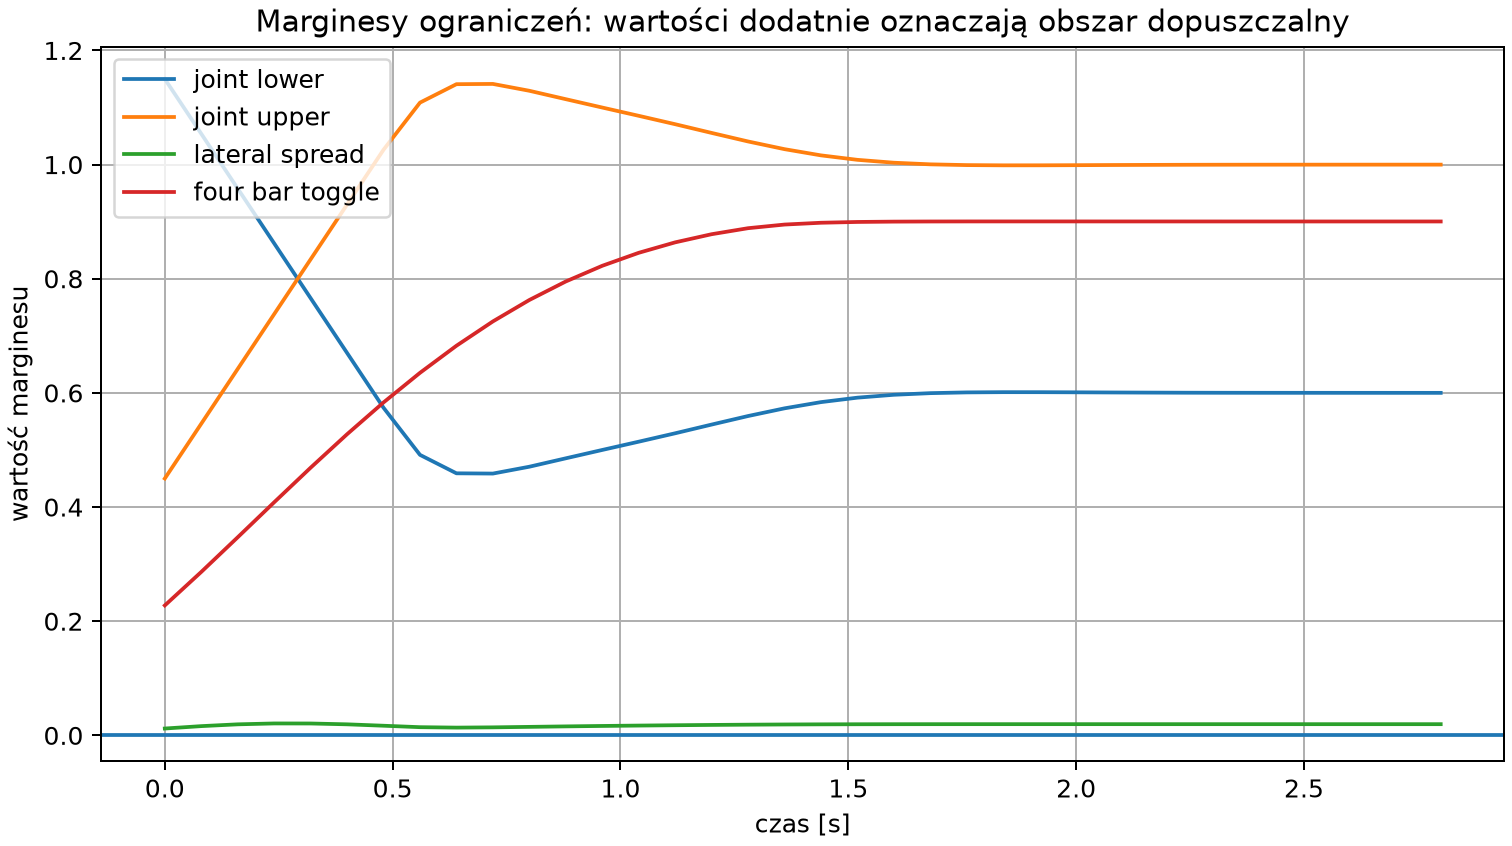
\includegraphics[width=\linewidth,height=0.50\textheight,keepaspectratio]{figures/mpc_safety_margins.png}
\end{columns}
\begin{block}{Docelowo}
Dodać moment, tarcie, kontakt i odzyskiwalność, a następnie sformułować warunki barierowe.
\end{block}
\note{Nie należy nazywać obecnych marginesów formalnymi gwarancjami. Ich wartość polega na tym, że tworzą mierzalny interfejs do przyszłych CBF i testów sprzętowych.}
\end{frame}

% 20
\begin{frame}{Rodzaje MPC używane w lokomocji}
\small
\begin{tabular}{p{0.29\textwidth}p{0.31\textwidth}p{0.30\textwidth}}
\toprule
\textbf{Rodzaj} & \textbf{Co upraszcza?} & \textbf{Po co?}\\
\midrule
Liniowe / wypukłe MPC & linearyzacja modelu, wypukłe ograniczenia & szybkie rozwiązywanie, prosty model\\[0.25em]
\midrule
Nieliniowe MPC & mniej uproszczeń w dynamice & lepsza dokładność, większy koszt obliczeń\\[0.25em]
\midrule
Centroidalne MPC & skupienie na środku masy i momencie pędu & dobre dla kontaktów i~równowagi\\[0.25em]
\midrule
MPC całego ciała & wszystkie przeguby i pełniejszy model & mniej warstw pośrednich, trudniejsze obliczenia\\[0.25em]
\midrule
MPC próbkowane & wiele kandydatów trajektorii & łatwe do zrównoleglenia, czasem mniej eleganckie matematycznie\\
\bottomrule
\end{tabular}
\source{Klasyczny przykład szybkiego wypukłego MPC: MIT Cheetah 3, Di Carlo i wsp., IROS 2018.}
\note{Użytkownik chciał zostawić ten slajd przed WBC i SRB. Należy tu podkreślić, że nie ma jednego „MPC”. Rodzina metod różni się modelem, solverem i miejscem w architekturze.}
\end{frame}

% 21
\begin{frame}{Chód jako harmonogram kontaktów}
\begin{columns}[T,onlytextwidth]
\column{0.48\textwidth}
\begin{itemize}
  \item Chód robota można opisać jako informację: która stopa dotyka podłoża w danym czasie.
  \item Harmonogram kontaktów decyduje, jakie siły wolno planować.
  \item Dla czworonoga typowe wzorce to stęp, kłus, galop, ale projekt badawczy może zacząć od prostszych sekwencji.
\end{itemize}
\column{0.48\textwidth}
\begin{center}
\begin{tikzpicture}[x=0.62cm,y=0.55cm]
  \foreach \r/\name in {0/FL,1/FR,2/RL,3/RR} {
    \node[font=\scriptsize] at (-0.6,-\r) {\name};
    \foreach \t in {0,...,7} {
      \pgfmathtruncatemacro{\contact}{mod(\t+\r,2)}
      \ifnum\contact=0
        \fill[safe!80] (\t,-\r) rectangle +(0.82,0.34);
      \else
        \fill[black!12] (\t,-\r) rectangle +(0.82,0.34);
      \fi
    }
  }
  \node[font=\scriptsize] at (3.4,-4.0) {zielone: kontakt, szare: przenoszenie};
\end{tikzpicture}
\end{center}
\end{columns}
\begin{block}{Rola MPC}
Dla zadanego harmonogramu kontaktów sterowanie predykcyjne dobiera ruch i siły tak, aby ciało pozostało stabilne i wykonalne.
\end{block}
\note{Tu można ostrożnie powiedzieć, że w pierwszym etapie harmonogram może być zadany z góry. Dopiero później można optymalizować także wybór kontaktów.}
\end{frame}

% 22
\begin{frame}{MPC dla humanoidów i psów: podobieństwa i różnice}
\scriptsize
\begin{tabular}{p{0.23\textwidth}p{0.32\textwidth}p{0.32\textwidth}}
\toprule
 & \textbf{Czworonóg} & \textbf{Humanoid}\\
\midrule
Kontakty & większa redundancja, więcej nóg w podporze & mniejszy wielokąt podparcia, częściej krytyczna równowaga\\[0.25em]
Priorytet & teren, odporność, sekwencje kontaktów & równowaga, manipulacja, koordynacja całego ciała\\[0.25em]
Model & często Single Rigid Body i siły kontaktu & często model centroidalny lub całego ciała\\[0.25em]
Ryzyko & poślizg, zahaczenie, złe ułożenie nogi & upadek, kontakt nieplanowany, sprzężenie z manipulacją\\
\bottomrule
\end{tabular}
\vspace{0.6em}
\begin{block}{Dlaczego to ważne dla projektu?}
\small Czworonóg jest praktycznym poligonem testowym dla idei potrzebnych także w~robocie humanoidalnym: kontaktu, predykcji, ograniczeń i bezpieczeństwa.
\end{block}
\note{Slajd powinien uspokoić odbiorców, że praca na czworonogu nie jest ślepą uliczką. To dobry testbed dla metod, które później skalują się do humanoidów.}
\end{frame}

% 23
\begin{frame}{Single Rigid Body: model pojedynczego ciała sztywnego}
\begin{block}{Single Rigid Body (SRB)}
Model pojedynczego ciała sztywnego traktuje korpus robota jako jedno ciało, a nogi głównie jako źródła sił kontaktowych.
\end{block}
\begin{columns}[T,onlytextwidth]
\column{0.48\textwidth}
\begin{itemize}
  \item Plus: prostszy, szybki, użyteczny dla planowania sił reakcji podłoża.
  \item Plus: popularny w czworonożnej lokomocji dynamicznej.
\end{itemize}
\column{0.48\textwidth}
\begin{itemize}
  \item Minus: pomija dużą część dynamiki nóg.
  \item Minus: nietypowa noga z mechanizmem czworoboku może wymagać dodatkowych ograniczeń niżej w sterowaniu.
\end{itemize}
\end{columns}
\source{Praktyczne implementacje SRB/MPC są dostępne np. w Quadruped-PyMPC.}
\note{Przy pierwszym użyciu podajemy pełną nazwę i dopiero potem skrót. Ważne: SRB nie rozwiąże automatycznie problemu rozstawionej nogi, bo może w ogóle nie widzieć szczegółów mechanizmu.}
\end{frame}

% 24
\begin{frame}{Whole-Body Control: sterowanie całym ciałem}
\begin{block}{Whole-Body Control (WBC)}
Sterowanie całym ciałem przekształca cele dla korpusu, stóp i sił kontaktowych na ruch lub momenty wszystkich przegubów.
\end{block}
\begin{center}
\begin{tikzpicture}[node distance=0.9cm,>=Latex]
  \tikzstyle{box}=[draw,rounded corners=2pt,fill=blue!6,minimum width=3.0cm,minimum height=0.72cm,align=center,font=\small]
  \node[box] (mpc) {Model Predictive\\Control};
  \node[box,right=of mpc] (wbc) {Whole-Body\\Control};
  \node[box,right=of wbc] (imp) {sterowanie\\impedancyjne};
  \node[box,right=of imp] (robot) {robot};
  \draw[->,thick] (mpc)--(wbc);
  \draw[->,thick] (wbc)--(imp);
  \draw[->,thick] (imp)--(robot);
\end{tikzpicture}
\end{center}
\begin{itemize}
  \item WBC może egzekwować zadania priorytetowe: kontakt, postawa, limity momentu, stabilizacja korpusu.
  \item Nowsze prace pokazują też MPC całego ciała z pełniejszą dynamiką, np. z MuJoCo.
\end{itemize}
\note{To powinien być slajd „gdzie to się wpina”. MPC może planować, WBC może realizować plan na wszystkich przegubach, a napędy mogą wykonywać warstwę impedancyjną.}
\end{frame}
